%\documentclass[12pt, twoside]{article}
%\documentclass[12pt]{article}%REMOVE AFTER
\documentclass[a4paper,14pt,oneside,openany]{extarticle}
\usepackage{a4wide}%REMOVE AFTER

%\usepackage{jmlda}
\usepackage[title]{appendix}%
\usepackage[utf8]{inputenc}
\usepackage[english, russian]{babel}
\usepackage[T2A]{fontenc}
\usepackage{lineno}
\usepackage{amssymb,amsfonts,amsmath,mathtext}
\usepackage{amsthm}
\usepackage{array}
%\usepackage{theorem}
\usepackage[all]{xy}
\usepackage{array}
\usepackage{multicol}
\usepackage{hhline}
\usepackage{graphicx}
\usepackage{float}
\usepackage{subcaption}
\usepackage{wrapfig}%Обтекание фигур (таблиц, картинок и прочего)
\usepackage{multirow}
\usepackage{pgfplots}
\pgfplotsset{compat=1.9}
\usepackage{graphicx}%
\usepackage{mathrsfs}%
\usepackage[title]{appendix}%
\usepackage{xcolor}%
\usepackage{textcomp}%
\usepackage{manyfoot}%
%\usepackage{booktabs}%
\usepackage{algorithm}%
\usepackage{algorithmicx}%
\usepackage{algpseudocode}%
\usepackage{listings}%
\graphicspath{{figures/}}  
\renewcommand{\thesubfigure}{\textit{\alph{subfigure}}}
\newcommand{\hdir}{.}

\theoremstyle{thmstylethree}
\newtheorem{definition}{Defenition}
\theoremstyle{thmstyletwo}
\newtheorem{remark}{Remark}

\theoremstyle{thmstyleone}
\newtheorem{theorem}{Theorem}
\newtheorem{lemma}{Lemma}

\raggedbottom
\begin{document}
%\English

\begin{center}
Федеральное государственное автономное образовательное учреждение\\ высшего образования\\
<<Московский физико-технический институт\\
(национальный исследовательский университет)>>\\
Физтех-школа прикладной математики и информатики\\
Кафедра интеллектуальных систем
\end{center}
%
\vspace{0pt plus5fill}
%
\begin{center}
\large{Терентьев Александр Александрович}
\end{center}
%
\vspace{0pt}
%
\begin{center}
\textbf{\large\MakeUppercase{Обратные задачи в моделировании нейронных дифференциальных уравнений в частных производных}}
\end{center}
%
\vspace{0pt}
%
\begin{center}
09.04.01~--- Информатика и вычислительная техника
\end{center}
%
\vspace{0pt}
%
\begin{center}
Выпускная квалификационная работа магистра
\end{center}
%
\vspace{0pt plus2fill}
%
\begin{center}
\hfill\parbox{8,4cm}{\textbf{Научный руководитель:}\\
Стрижов Вадим Викторович,\\
д-р физ.-мат. наук}\\
\vspace{0pt plus4fill}
Москва~--- 2026
\end{center}




%these fields are filled in by the journal editors
%\doi{10.21469/22233792}
%\receivedEng{January 01, 2017}

%\linenumbers

\section{Введение}

Обратная задача ЭЭГ имеет фундаментальное значение для исследования активности мозга, поскольку она
позволяет получить представление о пространственной и временной структуре распределения источников сигнала в мозге при выполнении
различных когнитивных и моторных задач. Это позволяет определять аномалии в активности мозга и их причины, 
что способствует пониманию внутренней работы мозга и выявлению областей с аномалиями проводимости, 
которые могут указывать на поврежденную ткань \cite{PascualMarqui1999}. 
Обратная задача ЭЭГ является плохо обусловленной, поэтому у нее не существует единственного
решения, обусловленного ограниченным числом наблюдений на поверхности головы.

Для восстановления приближённого решения необходимо задать модель источников и регуляризирующий функционал. 
В работах MNE \cite{Grech2008} и томографии электрической активности низкого разрешения (LORETA) \cite{Weinstein1999}
рассматриваются линейные источники и квадратичная регуляризация, учитывающие взаимосвязь между
источниками тока и измеренными потенциалами в предположении квазистатического приближения. 
Целью данной работы является предложить регуляризацию
для обратной задачи nPDE, основанную на максимально общей физической модели описания источников поля. 
Модель источников должна быть достаточно гибкой, чтобы описывать широкий спектр возможных источников сигнала в мозге, 
включая как локализованные, так и распределенные источники.
При этом регуляризация должна быть физически обоснованной, учитывать электромагнитную природу задачи 
и обеспечивать устойчивость решения.
В большинстве работ используется предположение о квазистатичности процессов, происходящих в мозге. 
В общем случае это неверно. Для моделирования источников коротких сигналов в мозге необходимо учитывать 
зависимость поля от скорости изменения источников сигнала. 
Целью работы является предложение такой модели, которая автоматически учитывается зависимость поля от 
скорости изменения источников сигнала, тем самым описывая эффект индукции от резкого изменения токов. 

\subsection{Определение задачи обратного восстановления ЭЭГ}

\begin{wrapfigure}{r}{0.25\textwidth}
 \centering
 \begin{minipage}[b]{0.25\textwidth}
     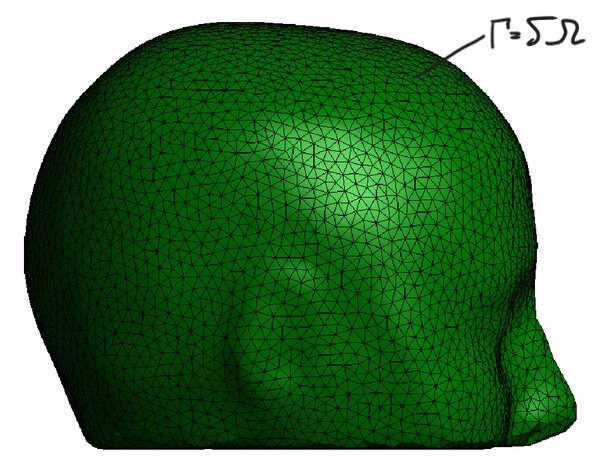
\includegraphics[width=\textwidth]{../../figures/head_surface_mesh.jpg}
     \caption{Поверхность головы $\Gamma$ }
     \label{fig: head_surface_mesh}
 \end{minipage}
 \hfill
 \begin{minipage}[b]{0.25\textwidth}
     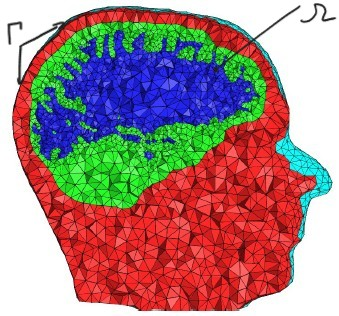
\includegraphics[width=\textwidth]{../../figures/head_mesh.jpg}  
     \caption{Рарез объема головы $\Omega$ }
     \label{fig: head_vulume_mesh}
 \end{minipage}
 
\end{wrapfigure}
В общем случае обратная задача ЭЭГ формулируется как задача восстановления
непрерывного распределения источников $s \in \mathcal{S}$ по конечному набору наблюдений $d \in \mathcal{O}$.
Введём три функциональных пространства:

Пространство источников $\mathcal{S}$ ~-- гильбертово пространство распределений поляризации $\mathbf{P}(\mathbf{r}, t)$ в области $\Omega \subset \mathbb{R}^3$.
Пространство полей $\mathcal{F}$ ~-- гильбертово пространство потенциалов $\phi(\mathbf{r}, t)$ и $\mathbf{A}(\mathbf{r}, t)$.
Пространство наблюдений $\mathcal{O} = \mathbb{R}^n$ ~-- евклидово пространство измерений на $n$ датчиках.

Пусть $T: \mathcal{S} \to \mathcal{F}$ ~-- оператор прямой задачи, ставящий в соответствие распределению источников поле, удовлетворяющее уравнениям Максвелла в области $\Omega$. Пусть $C: \mathcal{F} \to \mathcal{O}$ --- оператор наблюдения, проецирующий поле на значения, измеряемые датчиками на границе $\Gamma = \partial\Omega$. Тогда оператор наблюдаемой прямой задачи определяется как композиция:

\begin{equation}
    K = C \circ T: \mathcal{S} \to \mathcal{O}.
\end{equation}

Наблюдаемые данные $d$ представляются в виде:

\begin{equation}
    d = K s + \eta,
\end{equation}

где $\eta \in \mathcal{O}$ --- аддитивный шум. Требуется восстановить источник $s \in \mathcal{S}$ по данным $d \in \mathcal{O}$.
Оператор $K$ вырожден, так как множество источников, порождающих одинаковые наблюдения, бесконечно. Для корректной постановки задачи вводится регуляризация, обеспечивающая устойчивость и физическую обоснованность решения.

В задаче ЭЭГ $T$   является оператором решения уравнений Максвелла, который отображает распределение источников 
в электромагнитное поле. Из принципа суперпозициии и линейности уравнений Максвелла следует, что $T$ — линейный оператор.
Оператор $C$ который проецирует поле на значения, измеряемые датчиками. 
Поле $y=T s$ в модели является непрерывным по координатам $(x,y,z,t)$ в области головы $\Omega$. 
Однако наблюдения $d$ — это дискретные значения поля на датчиках, расположенных на поверхности головы $\Gamma$. 
Поэтому оператор $C$ — это дискретизирующий оператор, который отображает непрерывное поле в конечный набор значений на датчиках. 
В результате оператор $K=C T$ является композицией непрерывного оператора $T$ и дискретизирующего оператора $C$, 
что делает его вырожденным.

\section{Регулярпизация обратной задачи через энергию поля}

Из линейности оператора следует, что множество решений прямой задачи для данных $d$ задаётся 
$$\mathcal{X}(d)=\{x \in x_0 + \ker(K)\},~Kx_0=d.$$
Поэтому в качестве регуляризации предлагается взять квадратичный функционал, который моделирует энергию взаимодействия электромагнитного поля с источниками через положительно определённый оператор потенциала $T$:
\begin{equation}
    E[f] = \langle T f, f \rangle_{\mathcal{S}},
\end{equation}
где $Tf$ — поле, генерируемое источниками, а $f$ — сами источники.

Энергия поля задает слишком большую стоимость для решений, которые создают сильные поля на датчиках, что соответствует 
физической интуиции о том, что источники с высокой энергией менее вероятны. Но при этом она поощряет некомпактные решения,
которые не соответствуют реальным источникам в мозге. 
Поэтому в качестве дополнительного регуляризатора предлагается использовать функционал полной вариации $\mathrm{TV}(s)$, 
который поощряет локализованные и кусочно-постоянные решения.

Пусть $\mathcal{O}$ — гильбертово пространство наблюдений, $\mathcal{F}$ — гильбертово пространство полей, 
и $\mathcal{S}$ — гильбертово пространство источников.  Тогда задача восстановления источников формулируется 
как оптимизация функционала
\begin{equation}\label{eq:general_functional_full}
    J(s) = \|K s - d\|_{\mathcal{O}}^2 + \alpha \langle T s, s \rangle_{\mathcal{S}} + 
    \beta\,\mathrm{TV}(s) \rightarrow \min_{s\in\mathcal{S}},
\end{equation}
где первый член отвечает за соответствие данным, второй — за энергию взаимодействия поля с источниками и устойчивость модели,
а третий — за пространственную структурированность источника, $\alpha$ - регуляризация высокоэнергетических источников,
$\beta$ — регуляризация некомпактных источников. В случае, если решение $s$ представлено через нейросеть $s_\theta$,
эта постановка сводится к оптимизации по параметрам $\theta$.

На рисунке \ref{fig: LNN} показана упрощённая схема: оператор $D$ восстанавливает параметры источников из данных, 
а $G$ воспроизводит предсказанное поле. В operator-терминах $D$ задаёт обратное отображение из $\mathcal{O}$ в $\mathcal{S}$,
а $G$ реализует прямой оператор $K = C T$.

Таким образом, мы формулируем задачу nPDE как поиск решения $\hat{s}$ функционала \eqref{eq:general_functional_full} в 
пространстве $\mathcal{S}$. Оператор $K$ имеет ненулевое ядро, что приводит к бесконечному множеству решений, 
которые соответствуют данным $d$, а единственность достигается за счёт регуляризаторов $T$ и $\mathrm{TV}$.

\begin{figure}[H]
\centerline{
    \xymatrix{
    \chi_i: (N_x \times N_y \times N_z \times T)  \ar@{->}[rr]^-{D(\hat{s}|X, \mathcal{D})} && s \ar@{->}[rr]^-{G(\hat{X}|X(t), \hat{s}, \mathcal{D})} && \hat{\mathbf{X}}
    }
}
\caption{Модель сигнала ЭЭГ}
\label{fig: LNN}
\end{figure}

Формально пространственно-временной ряд $\chi$ можно записать как ряд поля $E(\mathbf{r})_t$. Таким образом задача состоит в нахождении в источниках поля $E$. 

В работе предлагается использовать уравнения в частных производных для восстановления динамики поля. В общем виде это можно записать так
$$A\left(s, r, t, E, \frac{\partial E}{\partial{\mathbf{r}}}, \frac{\partial E}{\partial{t}}, \vdots \right)= 0.$$
\section{Физико информированный подход}
Для физически обоснованных решений используется параметризация уравнений Максвелла через потенциалы и поляризацию. Нейросеть аппроксимирует в каждой точке $(x,y,z,t)$ семь компонент:

\[\phi,\ \mathbf{A}=(A_x,A_y,A_z),\ \mathbf{P}=(P_x,P_y,P_z).\]

Поляризация $\mathbf{P}$ определяет источники, потенциалы $\phi$ и $\mathbf{A}$ --- поля. Плотность заряда и плотность тока выражаются через поляризацию:

\begin{equation}
    \rho = -\operatorname{div} \mathbf{P},
    \qquad
    \mathbf{j} = \frac{\partial \mathbf{P}}{\partial t}.
\end{equation}

Электрическое поле $\mathbf{E}$ и магнитное поле $\mathbf{B}$ задаются через потенциалы:

\begin{equation}
    \mathbf{E} = -\nabla \phi - \frac{\partial \mathbf{A}}{\partial t},
    \qquad
    \mathbf{B} = \nabla \times \mathbf{A}.
\end{equation}

Параметризация через потенциалы и поляризацию минимизирует число степеней свободы и соответствует дипольной природе источников сигнала в мозге.

Уравнения Максвелла в выбранной постановке принимают вид волновых уравнений для потенциалов:

\begin{align}
    \square \phi &= 4\pi \nabla \cdot \mathbf{P}, \label{eq:wave_phi} \\
    \square \mathbf{A} &= -\frac{4\pi}{c} \frac{\partial \mathbf{P}}{\partial t}, \label{eq:wave_A}
\end{align}

где $\square = \nabla^2 - \frac{1}{c^2} \frac{\partial^2}{\partial t^2}$ --- оператор Д’Аламбера. Калибровка Лоренца:

\begin{equation}
    \nabla \cdot \mathbf{A} + \frac{1}{c} \frac{\partial \phi}{\partial t} = 0.
\end{equation}

Традиционная формулировка через поля $\mathbf{E}$, $\mathbf{B}$ и плотности $\rho$, $\mathbf{j}$ требует большего числа компонент и не обеспечивает естественной структуры поляризации. Решения уравнений Максвелла ищутся с помощью nPDE\cite{Zubov2021}.

\section{Операторная постановка и свойства операторов}
\label{sec:operator_properties}

\subsection{Оператор решения прямой задачи $T$}
Оператор $T: \mathcal{S} \to \mathcal{F}$ определяется как $T\mathbf{P} = (\phi, \mathbf{A})$, где $\phi$ и $\mathbf{A}$ --- решения волновых уравнений:

\begin{align}
    \square \phi &= 4\pi \nabla \cdot \mathbf{P}, \label{eq:wave_phi} \\
    \square \mathbf{A} &= -\frac{4\pi}{c} \frac{\partial \mathbf{P}}{\partial t}. \label{eq:wave_A}
\end{align}

Линейность оператора $T$ следует из линейности оператора Д’Аламбера $\square$ и линейности граничных условий. Для любых $\mathbf{P}_1, \mathbf{P}_2 \in \mathcal{S}$ и скаляров $\alpha, \beta \in \mathbb{R}$ выполняется:

\begin{equation}
    T(\alpha \mathbf{P}_1 + \beta \mathbf{P}_2) = \alpha T\mathbf{P}_1 + \beta T\mathbf{P}_2.
\end{equation}

Ограниченность оператора $T$ доказывается с использованием энергетических оценок для волновых уравнений. Рассмотрим норму решения $(\phi, \mathbf{A}) = T\mathbf{P}$ в пространстве $\mathcal{F}$:

\begin{equation}
    \|(\phi, \mathbf{A})\|_{\mathcal{F}}^2 = \int_\Omega \int_0^T \left( |\phi|^2 + \|\nabla \phi\|^2 + \|\mathbf{A}\|^2 + \|\nabla \times \mathbf{A}\|^2 + \left|\frac{\partial \mathbf{A}}{\partial t}\right|^2 \right) \, dt \, d\mathbf{r}.
\end{equation}

Для волнового уравнения $\square \phi = 4\pi \nabla \cdot \mathbf{P}$ с нулевыми начальными и граничными условиями справедлива оценка:

\begin{equation}
    \|\phi\|_{H^1(\Omega \times [0,T])} \leq C_1 \|\nabla \cdot \mathbf{P}\|_{L^2(\Omega \times [0,T])},
\end{equation}

где $C_1 > 0$ --- константа, зависящая от области $\Omega$ и временного интервала $[0,T]$, $H^1$ --- пространство Соболева. Аналогичная оценка справедлива для $\mathbf{A}$:

\begin{equation}
    \|\mathbf{A}\|_{H^1(\Omega \times [0,T])} \leq C_2 \left\|\frac{\partial \mathbf{P}}{\partial t}\right\|_{L^2(\Omega \times [0,T])}.
\end{equation}

Так как $\|\nabla \cdot \mathbf{P}\|_{L^2} \leq \|\mathbf{P}\|_{H^1}$ и $\left\|\frac{\partial \mathbf{P}}{\partial t}\right\|_{L^2} \leq \|\mathbf{P}\|_{H^1}$, то:

\begin{equation}
    \|T\mathbf{P}\|_{\mathcal{F}} \leq C_T \|\mathbf{P}\|_{\mathcal{S}},
\end{equation}

где $C_T = \max(C_1, C_2)$ --- константа, не зависящая от $\mathbf{P}$.

Положительная определённость оператора $T$ обусловлена физическим смыслом квадратичной формы $\langle T\mathbf{P}, \mathbf{P} \rangle_{\mathcal{S}}$, соответствующей энергии взаимодействия поля с источниками:

\begin{equation}
    \langle T\mathbf{P}, \mathbf{P} \rangle_{\mathcal{S}} = \int_\Omega \bigl(\rho \phi + \mathbf{A} \cdot \mathbf{j}\bigr) \, d\mathbf{r} > 0, \quad \forall \mathbf{P} \neq 0.
\end{equation}

\subsection{Оператор наблюдения $C$}
Оператор $C: \mathcal{F} \to \mathcal{O}$ определяется как:

\begin{equation}
    C(\phi, \mathbf{A}) = \bigl(\phi(\mathbf{r}_1, t), \phi(\mathbf{r}_2, t), \dots, \phi(\mathbf{r}_n, t)\bigr)^\top,
\end{equation}

где $\mathbf{r}_i \in \Gamma = \partial\Omega$ --- координаты датчиков. Оператор $C$ линеен и ограничен.

\subsection{Композиция операторов $K = C \circ T$}
Оператор $K: \mathcal{S} \to \mathcal{O}$ определяется как $K\mathbf{P} = C(T\mathbf{P})$. Оператор $K$ линеен, ограничен, и его ранг не превышает $n = \dim \mathcal{O}$.

\subsection{Апроксимация энергической регуляризации}
\label{subsec:regularization}
В работе в качестве регуляризации предлагается использовать энергию электрического поля, формально задаваемую как
\[ E = \int_{\Omega} \phi(r)\rho(r)\,dr. \]

Ее главным вычислительным недостатком является необходимость численного интегрирования по объему $\Omega$ на каждом шаге оптимизации,
и нахождение решениея nPDE для нее. Так как на каждом шаге оптимизации мы не можем гарантировать, что решение nPDE будет найдено 
с заданной точностью, то численное интегрирование может быть неточным и дорогим.Поэтому предлагается использовать стохастическую
аппроксимацию Монтекарло для оценки этого интеграла.

\begin{lemma}[Зквивалентность  энергии и Монте-Карло оценки через произведение $\phi\rho$]
Пусть $\Omega\subset\mathbb{R}^d$ — измеримое множество с конечным объёмом $|\Omega|>0$. Пусть функции $\phi,\rho:\Omega\to\mathbb{R}$ такие, что $\phi\rho\in L^1(\Omega)$. Пусть $r_1,\dots,r_K$ быть i.i.d. точками, выбранными по вероятностной мере $\mu$ на $\Omega$ с плотностью $p(r)>0$ почти всюду (в частности, допускается равномерная выборка $p\equiv1/|\Omega|$). Определим
\[ E:=\int_{\Omega}\phi(r)\rho(r)\,dr,\qquad \hat E_K:=\frac{1}{K}\sum_{i=1}^K w(r_i)\phi(r_i)\rho(r_i),\quad w(r)=\frac{1}{p(r)}.\]
Тогда выполняются следующие утверждения:
\begin{enumerate}
\item (Несмещённость) $\mathbb{E}[\hat E_K]=E$.
\item (Сходимость) $\hat E_K\xrightarrow{a.s.}E$ при $K\to\infty$; более того, при $\mathbb{E}[|w\phi\rho|]<\infty$ имеем $\hat E_K\to E$ в $L^1$.
\item (Случайная погрешность) Если дополнительно $w\phi\rho\in L^2(\mu)$, то по центральной предельной теореме
\[ \sqrt{K}(\hat E_K-E)\xrightarrow{d}\mathcal{N}(0,\sigma^2),\qquad \sigma^2=\mathrm{Var}_\mu(w\phi\rho). \]
Следовательно, типичный масштаб ошибки равен $O_p(1/\sqrt{K})$.
\item (Оценка хвостов) Если $|w(r)\phi(r)\rho(r)|\le M$ почти наверное, то по неравенству Хёффдинга для суммы независимых ограниченных слагаемых
\[ \mathbb{P}(|\hat E_K-E|\ge\varepsilon)\le 2\exp\Big(-\frac{2K\varepsilon^2}{M^2}\Big). \]
\end{enumerate}
\end{lemma}

\begin{proof}
Пункт 1: 
\[ \mathbb{E}[\hat E_K]=\mathbb{E}\Big[\frac{1}{K}\sum_{i=1}^K w(r_i)\phi(r_i)\rho(r_i)\Big]=\mathbb{E}[w(r)\phi(r)\rho(r)]=\int_{\Omega} \phi(r)\rho(r)\,dr=E, \]
где на втором шаге использована линейность матожидания и идентичность распределения сэмплов (см. \cite{Billingsley1995}).

Пункт 2: из предположения $\mathbb{E}[|w\phi\rho|]<\infty$ и закона больших чисел для i.i.d. последовательностей следует сходимость почти наверное $\hat E_K\to E$ и сходимость в среднем (при дополнительных условиях) --- в $L^1$ (см. \cite{Billingsley1995}).

Пункт 3: при конечной дисперсии $\mathrm{Var}_\mu(w\phi\rho)=\sigma^2<\infty$ применима центральная предельная теорема, которая даёт сходимость распределений к нормальной с указанной дисперсией (см. \cite{VanDerVaart1998}).

Пункт 4: если слагаемые ограничены по модулю $M$, то применима версия неравенства Хёффдинга для сумм i.i.d. ограниченных величин, откуда и следует указанная оценка (см. \cite{Hoeffding1963}).
\end{proof}


Для фиксированного множителя регуляризации $\lambda>0$ замена непрерывного регуляризатора $\lambda E$ на дискретную версию $\lambda\hat E_K$ даёт состоятельную аппроксимацию: $\hat E_K\to E$ при $K\to\infty$ и погрешность порядка $O_p(1/\sqrt{K})$.


\begin{remark}
Аппроксимация вида $\frac{1}{K}\sum_i\phi(r_i)\rho(r_i)$ (для $p\equiv 1/|\Omega|$) даёт простую и эффективную реализацию регуляризатора во время стохастического градиентного спуска и уменьшает вычислительные затраты по сравнению с оценкой полной энергии по сетке.
\end{remark}

\section{Теоретическая основа регуляризации через энергию}
\subsection{Постановка обратной задачи в операторной форме для конечного числа источников и датчиков}

Пусть $\Omega\subset\mathbb{R}^3$ — область, в которой заданы $m$ точечных источника с 
комплексными амплитудами $f_1,f_2, \vdots, f_m\in\mathbb{C}$ в точках $s_1,s_2, \vdots, s_m\in\Omega$. На фиксированной частоте
$\omega>0$ измеряется одна компонентa поля $E_z$ в двух точках $r_1,r_2, \vdots, r_n \notin\{s_1,s_2, \vdots, s_m\}$.
В дискретном приближении значение потенциала от источника описывается функцией $G(r,s;\omega)$:
\begin{equation}\label{eq:direct_em}
    d_i = G(r_i,s_1;\omega) f_1 + G(r_i,s_2;\omega) f_2 + \vdots + G(r_i,s_m;\omega) f_m,
    \qquad i=1,2, \vdots, n.
\end{equation}

Обозначим
\begin{equation}
    f=\begin{pmatrix}f_1\\ f_2 \\ \vdots \\ f_m\end{pmatrix},
    \qquad
    d=\begin{pmatrix}d_1\\ d_2 \\ \vdots \\ d_n\end{pmatrix},
    \qquad
    K=\begin{pmatrix}
        G(r_1,s_1;\omega) & G(r_1,s_2;\omega) & \cdots & G(r_1,s_m;\omega)\\
        G(r_2,s_1;\omega) & G(r_2,s_2;\omega) & \cdots & G(r_2,s_m;\omega)\\
        \vdots & \vdots & \ddots & \vdots\\
        G(r_n,s_1;\omega) & G(r_n,s_2;\omega) & \cdots & G(r_n,s_m;\omega)
    \end{pmatrix}.
\end{equation}
Тогда прямая задача записывается компактно как
\begin{equation}\label{eq:direct_matrix}
    d=Kf.
\end{equation}

Оператор $K$ является дискретной версией композиции $K=C T$, где $T$ — оператор решения уравнения Максвелла, 
а $C$ — оператор наблюдений на датчиках.

\subsection{Пример вырожденной геометрии и проблема неединственности}

Рассмотрим геометрию задачи для трех источников, 
при которой функции Грина для трех источников в двух точках наблюдения задаются следующей матрицей:
\begin{equation}\label{eq:degenerate_G}
    G(r_1,s_1)=g_{11}, G(r_2,s_1)=g_{21},
    G(r_1,s_2)=g_{12}, G(r_2,s_2)=g_{22},
    G(r_1,s_3)=g_{13}, G(r_2,s_3)=g_{23}.
\end{equation}
Тогда
\begin{equation}\label{eq:K_rank1}
    K=\begin{pmatrix}g_{11} & g_{12} & g_{13}\\ g_{21} & g_{22} & g_{23}\end{pmatrix},
    \qquad \mathrm{rank}(K)=2.
\end{equation}

Множество решений прямой задачи определяется в случае двух источников и двух датчиков как
\begin{equation}\label{eq:data_line}
    \mathcal{S}(d)=\{f\in\mathbb{C}^2: f_3 = \frac{f_1(g_{11}d_2 - g_{21}d_1) + f_2(g_{12}d_2-g_{22}d_1)}{g_{13}d_2-g_{23}d_1}\}.
\end{equation}
Это аффинное подпространство размерности один, и невырожденных решений бесконечно много. 
Формально, $\ker K=\{(x,y,z): a x+b y+c z=0\}$, и к любому решению можно прибавить произвольный элемент ядра, не изменяя данные.

\subsection{Функционал регуляризации и физика энергии}

Для устранения неединственности вводим регуляризованный функционал
\begin{equation}\label{eq:functional_basic}
    J(f)=\|K f-d\|_2^2 + \alpha \frac12 \|K f\|_2^2 + \beta (|f_1-f_2| + |f_1-f_3| + |f_2-f_3|),
    \qquad \alpha>0,\ \beta\ge0.
\end{equation}

Первое слагаемое это невязка между данными и оценки потенциала моделью. Второе слагаемое регуляризация энергии поля.
В частотной области оно эквивалентно квадратичному штрафу за амплитуду наблюдаемого поля. 
Третье слагаемое представляет собой дискретный вариант полной вариации,
поощряющий схожесть точечных источников и препятствующий неструктурированному разбросу амплитуд.

Подставляя матрицу \eqref{eq:K_rank1} и вводя вектор наблюдаемого поля
\begin{equation}\label{eq:field_observation}
    s = K f \in \mathbb{R}^2,
\end{equation}
функционал \eqref{eq:functional_basic} переписывается как
\begin{equation}\label{eq:functional_degenerate}
    J(f)=\|s-d\|_2^2 + \frac{\alpha}{2}\|s\|_2^2 + \beta \bigl(|f_1-f_2| + |f_1-f_3| + |f_2-f_3|\bigr),
    \qquad s=Kf.
\end{equation}

\subsubsection{Явное решение через минимизацию функционала}

Минимизируем функционал \eqref{eq:functional_basic} при $\beta=0$. Энергия взаимодействия представляет 
произведение источника на потенциал, генерируемый этим источником. В дискретном случае это скалярное 
произведение $f^T T^T f$, где $T$ — оператор потенциала:
\begin{equation}
    J(f) = \|Kf-d\|_2^2 + \frac{\alpha}{2}f^T T^T f.
\end{equation}

Раскроем функционал:
\begin{equation}
    J(f) = f^TK^TKf - 2f^TK^Td + \|d\|_2^2 + \frac{\alpha}{2}f^T T^T f.
\end{equation}

Вычислим градиент по $f$:
\begin{equation}
    \nabla_f J = 2K^TKf - 2K^Td + \alpha T^T f.
\end{equation}

Приравняв к нулю, получаем нормальную систему уравнений:
\begin{equation}\label{eq:normal_equations}
    (2K^TK + \alpha T^T)f^* = 2K^Td.
\end{equation}

Матрица $(2K^TK + \alpha T^T)$ размера $(3 \times 3)$ является положительно определённой при $\alpha > 0$, 
поскольку $K^TK$ положительно полуопределена (имеет ранг 2), а $T^T$ положитедльно определена, так как энергия 
поля $E[f] = f^T T^T f > 0$ при $f \neq 0$.
Таким образом, система имеет единственное решение $f^*$.

\textbf{Сравнение с исходным СЛАУ:} исходная система $Kf = d$ при $\mathrm{rank}(K) = 2$ имеет бесконечное 
множество решений, образующих одномерное аффинное подпространство:
\begin{equation}\label{eq:original_solution_set}
    \mathcal{F}_{\mathrm{original}} = \{f \in \mathbb{R}^3 : Kf = d\}.
\end{equation}

Регуляризованная задача с энергетическим штрафом $\alpha f^T T^T f > 0$ имеет единственное решение $f^*$, полученное как минимум функционала $J(f)$. 
Это решение, как правило, не принадлежит исходному множеству решений $\mathcal{F}_{\mathrm{original}}$ при $\alpha > 0$, так как энергетический штраф 
переводит оптимум в точку, которая генерирует наблюдаемое поле с иной амплитудой.

При $\alpha = 0$ (без энергетической регуляризации) система \eqref{eq:normal_equations} имеет нулевой правый оператор $(2K^TK)$, и множество решений 
совпадает с исходным: $\mathcal{F}^* = \mathcal{F}_{\mathrm{original}}$.

\subsection{Аналитическое решение в случае специальной геометрии}

Рассмотрим частный случай, где геометрия задачи и энергетический оператор $T$ допускают упрощённое решение. 
В частности, если источники расположены симметрично относительно датчиков, или матрица $T^T$ имеет блочную структуру, то система уравнений \eqref{eq:normal_equations} может быть решена в явном виде.

Для примера рассмотрим симметричный случай $f_1 = f_2 = x$ и $f_3 = 0$. Подставляя в нормальные уравнения:
\begin{equation}
    (2K^TK + \alpha T^T) \begin{pmatrix} x \\ x \\ 0 \end{pmatrix} = 2K^Td.
\end{equation}

Первые две компоненты уравнения (соответствующие $f_1$ и $f_2$) дают условия на $x$. 
Первое уравнение (строка 1 матрицы $(2K^TK + \alpha T^T)$):
\begin{equation}
    2\bigl[g_{11}(g_{11}+g_{12}) + g_{21}(g_{21}+g_{22})\bigr]x + \alpha (T^T)_{11} x = 2(g_{11}d_1 + g_{21}d_2).
\end{equation}

Второе уравнение (строка 2 матрицы):
\begin{equation}
    2\bigl[g_{12}(g_{11}+g_{12}) + g_{22}(g_{21}+g_{22})\bigr]x + \alpha (T^T)_{22} x = 2(g_{12}d_1 + g_{22}d_2).
\end{equation}

При предположении, что оператор $T^T$ также имеет симметрию, решение принимает форму:
\begin{equation}
    x = \frac{2(d_1+d_2)}{2(g_{11}+g_{12}) + \alpha \lambda_s},
\end{equation}
где $\lambda_s$ ~-- параметр, зависящий от оператора $T^T$.

\textbf{Физическая интерпретация:} энергетический штраф $\alpha f^T T^T f$ уменьшает амплитуду оптимального решения по сравнению с исходным СЛАУ (где $\alpha=0$). 
При $\alpha=0$ (отсутствие энергетической регуляризации) решение $f^*$ совпадает с одним из решений исходной системы $Kf = d$.
При возрастании $\alpha$ решение переходит в область, где энергия взаимодействия источников уменьшается, что физически соответствует поиску менее энергетичных источников.

\subsubsection{Аналитическое решение с TV регуляризацией}

Рассмотрим полный функционал с TV регуляризацией при $\beta > 0$:
\begin{equation}
    J(f) = \|Kf-d\|_2^2 + \frac{\alpha}{2}f^T T^T f + \beta (|f_1-f_2| + |f_1-f_3| + |f_2-f_3|).
\end{equation}

TV регуляризация вводит кусочно-гладкую структуру: она штрафует различия между компонентами источника, поощряя их группировку в однородные блоки.

Для симметричного случая $f_1 = f_2 = x$ и $f_3 = 0$ имеем:
\begin{equation}
    \mathrm{TV}(f) = |x-x| + |x-0| + |x-0| = 2|x|.
\end{equation}

Подставляя в функционал и опуская константы:
\begin{equation}
    J(x) = \left[(g_{11}+g_{12})x - d_1\right]^2 + \left[(g_{21}+g_{22})x - d_2\right]^2 + \frac{\alpha}{2} \lambda x^2 + 2\beta|x|,
\end{equation}
где $\lambda$ — энергетический параметр из оператора $T^T$ (зависит от геометрии).

Раскроем квадраты и соберём коэффициенты:
\begin{equation}
    J(x) = A x^2 - 2B x + 2\beta|x| + \text{const},
\end{equation}
где
\begin{equation}
    A = (g_{11}+g_{12})^2 + (g_{21}+g_{22})^2 + \frac{\alpha}{2} \lambda, \quad B = (g_{11}+g_{12})d_1 + (g_{21}+g_{22})d_2.
\end{equation}

\textbf{Случай 1: $x > 0$.} Функционал становится:
\begin{equation}
    J(x) = A x^2 - (2B - 2\beta) x + \text{const}.
\end{equation}
Условие минимума:
\begin{equation}
    \frac{dJ}{dx} = 2A x - (2B - 2\beta) = 0 \quad \Rightarrow \quad x^* = \frac{B - \beta}{A}.
\end{equation}
Это решение валидно, если $x^* > 0$, т.е. $B > \beta$.

\textbf{Случай 2: $x < 0$.} По симметрии задачи получаем $x^* = -\frac{B + \beta}{A}$, что требует $B < -\beta$. В физических приложениях обычно $B > 0$, поэтому этот случай редко встречается.

\textbf{Случай 3: $x = 0$.} Функция $|x|$ не дифференцируема в нуле. Используя субдифференциал:
\begin{equation}
    0 \in \partial J(0) \quad \Leftrightarrow \quad 0 \in [-2B - 2\beta, -2B + 2\beta].
\end{equation}
Это верно, если $B \leq \beta$.

\textbf{Итоговое решение при $\beta > 0$:}
\begin{equation}
    f^*_1 = f^*_2 = \begin{cases}
    \frac{B - \beta}{A}, & \text{если } B > \beta, \\[6pt]
    0, & \text{если } B \leq \beta,
    \end{cases} \quad f^*_3 = 0.
\end{equation}

Где:
\begin{equation}
    A = (g_{11}+g_{12})^2 + (g_{21}+g_{22})^2 + \frac{\alpha}{2} \lambda_s, \quad B = (g_{11}+g_{12})d_1 + (g_{21}+g_{22})d_2.
\end{equation}

\textbf{Физическая интерпретация с TV:} При увеличении коэффициента $\beta$ источники с малыми амплитудами 
занулятся, поощряя отбор самых значительных компонент. Пороговое значение $\beta$ определяет, 
при каком значении амплитуды источников они начинают зануляться.
Это соответствует разреживанию решения , что особенно важно в медицинских приложениях,
где источники активности в мозге локализованы и дискретны.

\subsection{Общая вариационная постановка}

Пусть $\mathcal{S},\mathcal{F},\mathcal{O}$ — гильбертовы пространства, $T:\mathcal{S}\to\mathcal{F}$ — 
линейный оператор перехода от источника к полю, $C:\mathcal{F}\to\mathcal{O}$ — линейный оператор 
наблюдения, и $K=C T:\mathcal{S}\to\mathcal{O}$ — линейный оператор прямой задачи. Пусть 
$T:\mathcal{S}\to\mathcal{F}$ — положительно определённый самосопряжённый оператор. Тогда предлагаемая вариационная задача формулируется как
\begin{equation}\label{eq:general_functional}
    J(s)=\|K s - d\|_{\mathcal{O}}^2 + \alpha \frac12 \langle T s, s\rangle_{\mathcal{S}} + \beta \,\mathrm{TV}(s),
    \qquad s\in \mathcal{S},
\end{equation}
где $\mathrm{TV}(s)$ — функционал полной вариации в пространстве источников.

Такое сочетание трёх членов имеет ясную физическую и математическую интерпретацию:
\begin{enumerate}
    \item $\|K f - d\|_{\mathcal{O}}^2$ обеспечивает соответствие данным;
    \item $\langle T f, f\rangle_{\mathcal{S}}$ моделирует энергию взаимодействия поля с источниками;
    \item $\mathrm{TV}(f)$ вводит структурную регуляризацию, поощряя локализованные и кусочно-постоянные 
    решения.
\end{enumerate}

\subsection{Единственность решения общей задачи}

\begin{lemma}\label{lem:operator_structure}
Пусть $\mathcal{S},\mathcal{F},\mathcal{O}$ — гильбертовы пространства, $T:\mathcal{S}\to\mathcal{F}$
 и $C:\mathcal{F}\to\mathcal{O}$ — ограниченные линейные операторы, $K=C\circ T:\mathcal{S}\to\mathcal{O}$
~-- их композиция. Если $T$ положительно определён на $\mathcal{S}$ 
(то есть $\langle Tf, f\rangle_{\mathcal{S}} > 0$ для всех $f \neq 0$), 
то оператор $A=K^*K+\alpha T$ (при $\alpha>0$) является положительно определённым и обратимым.
\end{lemma}

\begin{proof}[Доказательство леммы \ref{lem:operator_structure}]
Для любого $f \neq 0 \in \mathcal{S}$ имеем:
\begin{equation}
    \langle Af, f\rangle_{\mathcal{S}} = \langle K^*Kf, f\rangle_{\mathcal{S}} + 
    \alpha \langle Tf, f\rangle_{\mathcal{S}} = \|Kf\|_{\mathcal{O}}^2 + \alpha \langle Tf, f\rangle_{\mathcal{S}}.
\end{equation}
По предположению, $T>0$ означает $\langle Tf, f\rangle_{\mathcal{S}} \geq m_T \|f\|_{\mathcal{S}}^2$ для некоторого $m_T > 0$. Следовательно,
\begin{equation}
    \langle Af, f\rangle_{\mathcal{S}} \geq \alpha m_T \|f\|_{\mathcal{S}}^2 > 0,
\end{equation}
откуда следует положительная определённость $A$.
\end{proof}

\begin{theorem}\label{th:general_uniqueness}
Пусть $\mathcal{S},\mathcal{F}$ — гильбертовы пространства, $\mathcal{O} = \mathbb{R}^n$ ~-- 
евклидово пространство ($n$ — конечное число датчиков), $T:\mathcal{S}\to\mathcal{F}$ и 
$C:\mathcal{F}\to\mathcal{O}$ — ограниченные линейные операторы, 
$T$ — положительно определённый оператор. 
Пусть $\alpha>0$, $\beta\ge0$ и $\mathrm{TV}:\mathcal{S}\to[0,+\infty]$ — выпуклый
функционал. Тогда функционал \eqref{eq:general_functional} строго выпукл и имеет единственный 
глобальный минимум.
\end{theorem}

\begin{proof}
Разложим функционал и проанализируем каждый компонент, используя свойства операторов и 
конечномерность пространства наблюдений.

\textbf{Шаг 1: Анализ квадратичного компонента.}

Рассмотрим
\begin{equation}
    F(f)=\|K f - d\|_{\mathcal{O}}^2 + \frac{\alpha}{2}\langle T f, f\rangle_{\mathcal{S}}.
\end{equation}

Первый член — норма в конечномерном евклидовом пространстве $\mathcal{O} = \mathbb{R}^n$ (где $n$ — число датчиков). 
Её можно переписать через сопряжённый оператор $K^*:\mathcal{O}\to\mathcal{S}$:
\begin{equation}
    \|Kf-d\|_{\mathcal{O}}^2 = \langle Kf-d, Kf-d\rangle_{\mathcal{O}} = \langle K^*Kf, f\rangle_{\mathcal{S}} - 2\langle K^*d, f\rangle_{\mathcal{S}} + \|d\|_{\mathcal{O}}^2.
\end{equation}

Оператор $K^*K$ является композицией $K^*:\mathbb{R}^n\to\mathcal{S}$ и $K:\mathcal{S}\to\mathbb{R}^n$. Поскольку $\mathcal{O}=\mathbb{R}^n$
конечномерно, оператор $K^*K$ имеет \textbf{конечный ранг не выше} $n$. Он положительно полуопределён:
\begin{equation}
    \langle K^*K f, f\rangle_{\mathcal{S}} = \|Kf\|_{\mathcal{O}}^2 \geq 0 \quad \forall f \in \mathcal{S}.
\end{equation}

Второй член в $F$ — энергетический штраф. Поскольку $T$ положительно определён, имеем:
\begin{equation}
    \langle T f, f\rangle_{\mathcal{S}} > 0 \quad \forall f \neq 0 \in \mathcal{S}.
\end{equation}

\textbf{Шаг 2: Строгая выпуклость $F$ и роль конечномерности.}

Функционал $F$ квадратичен:
\begin{equation}
    F(f) = \langle A f, f\rangle_{\mathcal{S}} - 2\langle b, f\rangle_{\mathcal{S}} + c,
\end{equation}
где $A = K^*K + \frac{\alpha}{2}T$, $b = K^*d$, $c = \|d\|_{\mathcal{O}}^2$.

Ключевое свойство: оператор $A$ является суммой оператора $K^*K$ (конечного ранга, положительно полуопределённого) и оператора $\frac{\alpha}{2}T$ 
(положительно определённого на всём $\mathcal{S}$). При $\alpha > 0$ энергетический оператор $T$ дополняет ранга оператора $K^*K$ до полного ранга.
 Для любого $f \neq 0$:
\begin{equation}
    \langle A f, f\rangle_{\mathcal{S}} = \langle K^*K f, f\rangle_{\mathcal{S}} + \frac{\alpha}{2}\langle T f, f\rangle_{\mathcal{S}} \geq \frac{\alpha}{2} m_T \|f\|_{\mathcal{S}}^2 > 0,
\end{equation}
где $m_T > 0$ — константа такой, что $\langle T f, f\rangle_{\mathcal{S}} \geq m_T \|f\|_{\mathcal{S}}^2$ для всех $f \in \mathcal{S}$ (существует по положительной определённости $T$). Таким образом, оператор $A$ положительно определён, и квадратичный функционал $F$ строго выпуклый.

\textbf{Шаг 3: Свойства полной вариации.}

Функционал полной вариации $\mathrm{TV}:\mathcal{S}\to[0,+\infty]$ по определению выпуклый: для всех $f_1, f_2 \in \mathcal{S}$ и $\lambda \in [0,1]$:
\begin{equation}
    \mathrm{TV}(\lambda f_1 + (1-\lambda)f_2) \leq \lambda \,\mathrm{TV}(f_1) + (1-\lambda)\,\mathrm{TV}(f_2).
\end{equation}
Кроме того, $\mathrm{TV}$ является нижнеполунепрерывным функционалом в слабой топологии пространства $\mathcal{S}$.

\textbf{Шаг 4: Строгая выпуклость суммы.}

Сумма 
\begin{equation}
    J(f) = F(f) + \beta \,\mathrm{TV}(f)
\end{equation}
при $\beta \geq 0$ остаётся строго выпуклой, поскольку $F$ строго выпукла. Для всех $f_1 \neq f_2$ и $\lambda \in (0,1)$:
\begin{equation}
    J(\lambda f_1 + (1-\lambda)f_2) < \lambda J(f_1) + (1-\lambda)J(f_2).
\end{equation}


\textbf{Шаг 5: Коэрцитивность и существование минимума.}

Функционал $J$ коэрцитивен: $J(f) \to +\infty$ при $\|f\|_{\mathcal{S}} \to \infty$. Это следует из того, что:
\begin{equation}
    J(f) \geq \langle K^*K f, f\rangle_{\mathcal{S}} + \frac{\alpha}{2}\langle T f, f\rangle_{\mathcal{S}} - 
    2\|K^*d\|_{\mathcal{S}} \|f\|_{\mathcal{S}} \geq c_1 \|f\|_{\mathcal{S}}^2 - c_2 \|f\|_{\mathcal{S}},
\end{equation}
где $c_1 > 0$ — константа положительной определённости $A$, а $c_2$ — ограниченная константа.

Поскольку $J$ строго выпуклый, нижнеполунепрерывный и коэрцитивный на гильбертовом пространстве $\mathcal{S}$, 
он имеет \textit{единственный} глобальный минимум $f^* \in \mathcal{S}$.
\end{proof}

\begin{remark}
Теорема \ref{th:general_uniqueness} подчёркивает ключевую роль энергетического члена $\frac{\alpha}{2}\langle Tf, 
f\rangle_{\mathcal{S}}$ в обеспечении единственности решения, особенно в контексте конечного числа датчиков.

\begin{enumerate}
    \item \textbf{Конечномерность пространства наблюдений:}
    Поскольку $\mathcal{O} = \mathbb{R}^n$ (где $n$ — число датчиков),
    оператор $K^*K$ имеет конечный ранг, не превышающий $n$. Это означает, что ядро оператора $K$ может быть нетривиальным и иметь размерность $\dim \ker K = \dim \mathcal{S} - \mathrm{rank}(K) \geq \dim \mathcal{S} - n$. В частности, при $\dim \mathcal{S} > n$ (пространство источников имеет большую размерность, чем пространство наблюдений) задача автоматически становится недоопределённой.
    
    \item \textbf{Роль энергетического оператора $T$:}
    Энергетический штраф $\alpha \langle Tf, f\rangle_{\mathcal{S}}$ 
    полностью определён на гильбертовом пространстве $\mathcal{S}$ и не зависит от конечномерности $\mathcal{O}$. Благодаря положительной определённости $T$, 
    оператор $A = K^*K + \frac{\alpha}{2}T$ остаётся положительно определённым, несмотря на ранг оператора $K$. 
    Это гарантирует строгую выпуклость функционала $F$ на всём пространстве $\mathcal{S}$.
    
    \item \textbf{Недостаточность одной регуляризации:} 
    Без энергетического члена ($\alpha=0$): при $\dim \mathcal{S} > n$ функционал $\|Kf-d\|_{\mathcal{O}}^2$ имеет 
    бесконечномерное множество решений (полное аффинное подпространство размерности $\dim \mathcal{S} - n > 0$). 
    Даже добавление TV-регуляризации $\beta\,\mathrm{TV}(f)$ не обеспечивает единственность.
    Без структурной регуляризации ($\beta=0$): решение физически неправдоподобное и
    излишне гладкое в пространстве источников.

    
    \item \textbf{Регуляризация при конечном числе датчиков:} Энергетический член обепечивает единственность решения, компенсируя
    конечномерности наблюдений, добавляет бесконечномерно ограничение в виде положительно определённой формы, 
    а TV-регуляризация добавляет структурные ограничения. Вместе они обеспечивают как математическую корректность (единственность, устойчивость), 
    так и физическую обоснованность решения.
    
\end{enumerate}
\end{remark}

\subsection{Анализ аппроксимации оператора прямой задачи}

На практике оператор $T$ часто аппроксимируется последовательностью $T_n$ (например, численным решателем или обучаемым суррогатом). Рассмотрим функционалы
\begin{equation}
    J_n(f)=\|C T_n f - d\|_{\mathcal{O}}^2 + \frac{\alpha}{2} \langle T_n f, f\rangle_{\mathcal{S}} + \beta \mathrm{TV}(f),
\end{equation}
где $\mathcal{S}, \mathcal{F}, \mathcal{O}$ — гильбертовы пространства, $T, T_n: \mathcal{S} \to \mathcal{F}$ — ограниченные линейные операторы, $C: \mathcal{F} \to \mathcal{O}$ — ограниченный линейный оператор наблюдения, $\alpha>0$, $\beta\ge0$, а $\mathrm{TV}: \mathcal{S} \to [0,+\infty]$ — выпуклый нижнеполунепрерывный функционал. Оператор $T$ является положительно определённым оператором потенциала: существует $m_T > 0$ такое, что $\langle T f, f\rangle_{\mathcal{S}} \ge m_T \|f\|_{\mathcal{S}}^2$ для всех $f \in \mathcal{S}$. Квадратичная форма $\langle T f, f\rangle_{\mathcal{S}}$ соответствует энергии взаимодействия поля с источниками.

\begin{theorem}[Сходимость минимизаторов]
Пусть выполнены следующие условия:
\begin{enumerate}
    \item $T_n \to T$ равномерно на ограниченных множествах $\mathcal{S}$, то есть $\forall R>0$: $\sup_{\|f\|_{\mathcal{S}} \le R} \|T_n f - T f\|_{\mathcal{F}} \to 0$ при $n\to\infty$.
    \item Существует $M>0$ такое, что $\sup_n \|T_n\|_{\mathcal{L}(\mathcal{S},\mathcal{F})} \le M$ (равномерная ограниченность).
    \item Оператор $C: \mathcal{F} \to \mathcal{O}$ ограничен.
    \item Оператор $T$ положительно определён: $\exists m_T>0$ такое, что $\langle T f, f\rangle_{\mathcal{S}} \ge m_T \|f\|_{\mathcal{S}}^2$ для всех $f \in \mathcal{S}$ (коэрцитивность энергетического члена).
    \item Функционал $\mathrm{TV}$ ограничен снизу и коэрцитивен: $\mathrm{TV}(f) \ge c \|f\|_{\mathcal{S}} - d$ для некоторых $c>0, d\ge0$.
\end{enumerate}
Обозначим $J(f) = \|C T f - d\|_{\mathcal{O}}^2 + \frac{\alpha}{2} \langle T f, f\rangle_{\mathcal{S}} + \beta \mathrm{TV}(f)$.
Пусть $f_n^*$ — единственный глобальный минимум $J_n$, а $f^*$ — единственный глобальный минимум $J$.
Тогда $f_n^* \to f^*$ сильно в норме $\mathcal{S}$ при $n\to\infty$.
\end{theorem}

\begin{proof}
\textbf{1. Коэрцитивность и ограниченность.}
Для любого $f \in \mathcal{S}$ имеем
\begin{align*}
    J_n(f) &\ge \|C T_n f - d\|_{\mathcal{O}}^2 + \frac{\alpha}{2} \langle T_n f, f\rangle_{\mathcal{S}} + \beta \mathrm{TV}(f) \\
    &\ge \frac{\alpha}{2} \langle T_n f, f\rangle_{\mathcal{S}} + \beta (c \|f\|_{\mathcal{S}} - d).
\end{align*}
Так как семейство $\{T_n\}$ равномерно ограничено, существует константа $C_1>0$ такая, что $|\langle T_n f, f\rangle_{\mathcal{S}}| \le C_1 \|f\|_{\mathcal{S}}^2$.
По условию (4) для точного оператора $T$ имеем $\langle T f, f\rangle_{\mathcal{S}} \ge m_T \|f\|_{\mathcal{S}}^2$.
В силу равномерной сходимости $T_n \to T$ на шарах, можно показать, что существует $N$ и $\tilde{m}>0$ такие, что для всех $n \ge N$ и всех $f \in \mathcal{S}$:
\begin{equation}
    \langle T_n f, f\rangle_{\mathcal{S}} \ge \tilde{m} \|f\|_{\mathcal{S}}^2.
\end{equation}
Следовательно, для больших $n$ функционалы $J_n$ коэрцитивны:
\begin{equation}
    J_n(f) \ge \frac{\alpha}{2} \tilde{m} \|f\|_{\mathcal{S}}^2 + \beta c \|f\|_{\mathcal{S}} - \beta d - C_2 \to +\infty \quad \text{при } \|f\|_{\mathcal{S}} \to \infty.
\end{equation}
Поскольку $J_n(f_n^*) \le J_n(0) = \|d\|_{\mathcal{O}}^2 + \beta \mathrm{TV}(0) < \infty$, последовательность $\{f_n^*\}$ ограничена в $\mathcal{S}$.

\textbf{2. Слабая сходимость подпоследовательности.}
Так как $\mathcal{S}$ рефлексивно, из ограниченной последовательности можно выделить слабо сходящуюся подпоследовательность (обозначаем её также $\{f_n^*\}$): $f_n^* \rightharpoonup \bar f$ в $\mathcal{S}$.

\textbf{3. Нижний предел функционалов.}
Функционал $f \mapsto \|C T f - d\|_{\mathcal{O}}^2$ непрерывен по сильной топологии и, следовательно, слабо нижнеполунепрерывен.
Функционал $f \mapsto \langle T f, f\rangle_{\mathcal{S}}$ является квадратичной формой, соответствующей ограниченному самосопряженному оператору $T$ (так как $T$ положительно определён), и также слабо нижнеполунепрерывен.
Функционал $\mathrm{TV}$ по условию слабо нижнеполунепрерывен.
Сумма слабо нижнеполунепрерывных функционалов является слабо нижнеполунепрерывной. Поэтому
\begin{equation}
    J(\bar f) \le \liminf_{n\to\infty} J(f_n^*).
\end{equation}

\textbf{4. Оценка $\limsup$.}
Так как $f_n^*$ — минимум $J_n$, для любого $f \in \mathcal{S}$ (в частности для $f^*$) имеем $J_n(f_n^*) \le J_n(f^*)$. Значит,
\begin{equation}
    \limsup_{n\to\infty} J_n(f_n^*) \le \limsup_{n\to\infty} J_n(f^*).
\end{equation}
Поскольку $T_n \to T$ равномерно на ограниченных множествах, а $f^*$ фиксирован, $T_n f^* \to T f^*$ сильно в $\mathcal{F}$. Тогда $\|C T_n f^* - d\|_{\mathcal{O}}^2 \to \|C T f^* - d\|_{\mathcal{O}}^2$ и $\langle T_n f^*, f^*\rangle_{\mathcal{S}} \to \langle T f^*, f^*\rangle_{\mathcal{S}}$. Следовательно, $\limsup_{n\to\infty} J_n(f^*) = J(f^*)$.

\textbf{5. Предел.}
Собираем неравенства:
\begin{equation}
    J(\bar f) \le \liminf_{n\to\infty} J_n(f_n^*) \le \limsup_{n\to\infty} J_n(f_n^*) \le J(f^*).
\end{equation}
Так как $f^*$ — единственный глобальный минимум $J$, имеем $J(\bar f) \ge J(f^*)$. Отсюда $J(\bar f) = J(f^*)$ и $\bar f = f^*$.

\textbf{6. Сильная сходимость.}
Все слабые предельные точки последовательности $\{f_n^*\}$ совпадают с $f^*$, следовательно, $f_n^* \rightharpoonup f^*$ в $\mathcal{S}$.
Остаётся доказать сильную сходимость. Рассмотрим разность:
\begin{align*}
    \frac{\alpha}{2} \langle T_n f_n^*, f_n^*\rangle_{\mathcal{S}} - \frac{\alpha}{2} \langle T f^*, f^*\rangle_{\mathcal{S}}
    =& J_n(f_n^*) - \|C T_n f_n^* - d\|_{\mathcal{O}}^2 - \beta \mathrm{TV}(f_n^*) \\
    &- \bigl( J(f^*) - \|C T f^* - d\|_{\mathcal{O}}^2 - \beta \mathrm{TV}(f^*) \bigr).
\end{align*}
Так как $J_n(f_n^*) \to J(f^*)$ (из цепочки неравенств выше), $\|C T_n f_n^* - d\|_{\mathcal{O}}^2 \to \|C T f^* - d\|_{\mathcal{O}}^2$ (по слабой сходимости и компактности: $T_n f_n^* = (T_n - T) f_n^* + T f_n^*$. Первое слагаемое стремится к нулю по равномерной сходимости $T_n \to T$ на ограниченных множествах, второе слабо сходится к $T f^*$. Тогда $C T_n f_n^* \rightharpoonup C T f^*$ в $\mathcal{O}$, а норма квадрата слабо нижнеполунепрерывна, но предел значений известен. Можно использовать стандартный аргумент: если $u_n \rightharpoonup u$ и $\|u_n\| \to \|u\|$, то $u_n \to u$ сильно. Здесь $u_n = C T_n f_n^*$, $u = C T f^*$. Равенство пределов норм следует из сходимости значений функционалов.) и $\mathrm{TV}(f_n^*) \to \mathrm{TV}(f^*)$ (так как $\mathrm{TV}$ слабо нижнеполунепрерывен и пределы совпадают), получаем
\begin{equation}
    \langle T_n f_n^*, f_n^*\rangle_{\mathcal{S}} \to \langle T f^*, f^*\rangle_{\mathcal{S}}.
\end{equation}
Разложим:
\begin{equation}
    \langle T_n f_n^*, f_n^*\rangle_{\mathcal{S}} = \langle T f_n^*, f_n^*\rangle_{\mathcal{S}} + \langle (T_n - T) f_n^*, f_n^*\rangle_{\mathcal{S}}.
\end{equation}
Второе слагаемое стремится к нулю, так как $\| (T_n - T) f_n^*\|_{\mathcal{F}} \to 0$ (равномерная сходимость на ограниченных множествах).
Следовательно, $\langle T f_n^*, f_n^*\rangle_{\mathcal{S}} \to \langle T f^*, f^*\rangle_{\mathcal{S}}$.
Так как форма $\langle T \cdot, \cdot\rangle_{\mathcal{S}}$ коэрцитивна (условие 4), это влечёт сильную сходимость $f_n^* \to f^*$ в $\mathcal{S}$.
\end{proof}

\subsection{Схема решения обратной задачи}

Рассмотрим обратную задачу восстановления распределения источников $s \in \mathcal{S}$ по наблюдаемым данным $d \in \mathcal{O}$ в рамках операторной постановки $d = Ks + \eta$, где $K = C \circ T$ --- композиция оператора решения прямой задачи $T: \mathcal{S} \to \mathcal{F}$ и оператора наблюдения $C: \mathcal{F} \to \mathcal{O}$. Для обеспечения единственности и устойчивости решения вводится регуляризованный функционал:

\begin{equation}
    J(s) = \|Ks - d\|_{\mathcal{O}}^2 + \alpha \mathcal{R}_E(s) + \beta \mathcal{R}_{TV}(s),
\end{equation}

где $\mathcal{R}_E(s) = \langle Ts, s \rangle_{\mathcal{S}}$ --- энергетический регуляризатор, $\mathcal{R}_{TV}(s)$ --- функционал полной вариации, $\alpha > 0$ и $\beta \geq 0$ --- параметры регуляризации.

\subsubsection{Аппроксимация оператора прямой задачи и сходимость решений}

Пусть оператор прямой задачи $T$ аппроксимируется последовательностью операторов $T_n: \mathcal{S} \to \mathcal{F}$, сходящихся к $T$ в равномерной операторной топологии на ограниченных множествах. Введём аппроксимированный оператор наблюдения $K_n = C \circ T_n$ и соответствующий регуляризованный функционал:

\begin{equation}
    J_n(s) = \|K_n s - d\|_{\mathcal{O}}^2 + \alpha \langle T_n s, s \rangle_{\mathcal{S}} + \beta \mathcal{R}_{TV}(s).
\end{equation}

Минимизация функционала $J_n(s)$ по $s \in \mathcal{S}$ эквивалентна решению вариационной задачи:

\begin{equation}
    s_n^* = \arg\min_{s \in \mathcal{S}} J_n(s).
\end{equation}

Сходимость аппроксимированных решений $s_n^*$ к точному решению $s^*$ при $n \to \infty$ обеспечивается теоремой о сходимости минимизаторов (см. раздел \ref{subsec:regularization}).

\subsubsection{Энергетическая регуляризация и её свойства}

Энергетический регуляризатор $\mathcal{R}_E(s) = \langle Ts, s \rangle_{\mathcal{S}}$ вводится как квадратичная форма, соответствующая положительно определённому оператору потенциала $T$. В контексте электромагнитных задач эта форма интерпретируется как энергия взаимодействия поля с источниками:

\begin{equation}
    \mathcal{R}_E(s) = \int_{\Omega} \bigl(\rho(\mathbf{r}) \phi(\mathbf{r}) + \mathbf{A}(\mathbf{r}) \cdot \mathbf{j}(\mathbf{r})\bigr) \, d\mathbf{r},
\end{equation}

где $\rho = -\operatorname{div} \mathbf{P}$ --- плотность заряда, $\mathbf{j} = \partial_t \mathbf{P}$ --- плотность тока, $\phi$ и $\mathbf{A}$ --- скалярный и векторный потенциалы, $\mathbf{P}$ --- поляризация.

Свойства энергетического регуляризатора:
\begin{enumerate}
    \item \textbf{Положительная определённость}: $\mathcal{R}_E(s) > 0$ для всех $s \neq 0$, что обеспечивает строгую выпуклость функционала $J(s)$.
    \item \textbf{Физическая интерпретация}: минимизация $\mathcal{R}_E(s) = \langle Ts, s \rangle_{\mathcal{S}}$ соответствует поиску решений с минимальной энергией взаимодействия поля с источниками, что согласуется с принципом наименьшего действия в электродинамике.
    \item \textbf{Устойчивость}: при $\alpha > 0$ функционал $J(s)$ коэрцитивен и имеет единственный минимум даже в случае вырожденного оператора $K$.
\end{enumerate}

\subsubsection{Структурная регуляризация и функционал полной вариации}

Функционал полной вариации $\mathcal{R}_{TV}(s)$ вводится для подавления нефизичных осцилляций в решении и поощрения кусочно-постоянных распределений источников. В непрерывном случае он определяется как:

\begin{equation}
    \mathcal{R}_{TV}(s) = \int_{\Omega} \|\nabla s(\mathbf{r})\| \, d\mathbf{r}.
\end{equation}

В дискретной постановке функционал аппроксимируется суммой по пространственным производным плотности заряда $\rho = -\operatorname{div} \mathbf{P}$:

\begin{equation}
    \mathcal{R}_{TV}(s) \approx \frac{1}{|\Omega|} \int_{\Omega} \sqrt{\|\nabla \rho(\mathbf{r})\|^2 + \varepsilon} \, d\mathbf{r},
\end{equation}

где $\varepsilon > 0$ --- малый параметр, обеспечивающий дифференцируемость функционала.

Свойства функционала полной вариации:
\begin{enumerate}
    \item \textbf{Выпуклость}: $\mathcal{R}_{TV}(s)$ --- выпуклый функционал, что гарантирует существование единственного минимума при $\beta > 0$.
    \item \textbf{Разреживание}: минимизация $\mathcal{R}_{TV}(s)$ способствует локализации источников и подавлению малых флуктуаций, что соответствует физической природе источников сигнала в мозге.
    \item \textbf{Устойчивость к шуму}: функционал устойчив к высокочастотным шумам в данных, что критически важно для задач ЭЭГ.
\end{enumerate}

\subsubsection{Метод минимизации регуляризованного функционала}

Минимизация функционала $J(s)$ осуществляется методом градиентного спуска в гильбертовом пространстве $\mathcal{S}$. Градиент функционала $J(s)$ по $s$ вычисляется как:

\begin{equation}
    \nabla_s J(s) = 2K^*(Ks - d) + \alpha T^* s + \beta \partial \mathcal{R}_{TV}(s),
\end{equation}

где $K^*$ --- сопряжённый оператор к $K$, $T^*$ --- сопряжённый оператор к $T$, $\partial \mathcal{R}_{TV}(s)$ --- субдифференциал функционала полной вариации.

Для численной реализации градиентного спуска вводится последовательность итераций:

\begin{equation}
    s^{(k+1)} = s^{(k)} - \gamma_k \nabla_s J(s^{(k)}),
\end{equation}

где $\gamma_k > 0$ --- шаг градиентного спуска, выбираемый из условия монотонного убывания функционала $J(s^{(k)})$. 
Сходимость итерационного процесса к единственному минимуму $s^*$ обеспечивается теоремой о сходимости 
градиентного спуска для строго выпуклых функционалов.


\subsubsection{Адаптивная регуляризация и барьерные методы}

Для обеспечения устойчивости численного решения вводится барьерная функция, релаксирующая жёсткое ограничение $Ks = d$:

\begin{equation}
    \mathcal{B}(s) = \lambda_{\mathrm{data}} \bigl(T + \alpha_{\mathrm{data}} T^2\bigr),
    \quad T = \|Ks - d\|_{\mathcal{O}}^2 + \lambda_{\mathrm{time}} \|\partial_t (Ks - d)\|_{\mathcal{O}}^2,
\end{equation}

где $\lambda_{\mathrm{data}} > 0$ --- параметр барьерной функции, $\alpha_{\mathrm{data}} > 0$ --- коэффициент квадратичного штрафа, $\lambda_{\mathrm{time}} \geq 0$ --- вес временной регуляризации.

Адаптивная настройка параметра $\lambda_{\mathrm{data}}$ осуществляется на основе мониторинга скорости убывания функционала $J(s)$. Если улучшение функционала замедляется, $\lambda_{\mathrm{data}}$ увеличивается для усиления соответствия данным; в противном случае --- уменьшается для предоставления большей свободы регуляризаторам. Такой подход обеспечивает баланс между точностью аппроксимации данных и устойчивостью решения.

\subsubsection{Теоретическое обоснование сходимости алгоритма}

Сходимость предложенного алгоритма обосновывается следующими положениями:
\begin{enumerate}
    \item \textbf{Сходимость аппроксимированных операторов}: при $T_n \to T$ минимизаторы $s_n^*$ функционалов $J_n(s)$ сходятся к минимизатору $s^*$ функционала $J(s)$.
    \item \textbf{Единственность решения}: при $\alpha > 0$ и положительно определённом операторе $T$ функционал $J(s)$ строго выпукл и имеет единственный минимум.
    \item \textbf{Устойчивость к шуму}: регуляризаторы $\mathcal{R}_E(s)$ и $\mathcal{R}_{TV}(s)$ обеспечивают устойчивость решения к аддитивному шуму $\eta$ в данных.
    \item \textbf{Физическая согласованность}: энергетический регуляризатор $\mathcal{R}_E(s)$ гарантирует, что решение соответствует принципам электродинамики, а функционал полной вариации $\mathcal{R}_{TV}(s)$ --- структурным особенностям источников сигнала в мозге.
\end{enumerate}

Таким образом, предложенная алгоритмическая схема обеспечивает корректное решение обратной задачи ЭЭГ в рамках физико-информированного подхода, 
сочетая общность решения с физической интерпретируемостью результатов.

Сначала реализуется барьерное приближение условия $Kf=d$, затем условие смягчается и уточняется оператор наблюдения $K$ аппроксимируемый nPDE. Параметры $\lambda_{\mathrm{data}}$, 
$\alpha_{\mathrm{data}}$ и $\lambda_{\mathrm{time}}$ адаптивно 
настраиваются в процессе оптимизации для обеспечения баланса между точностью аппроксимации данных и устойчивостью решения. При этом достигается сходимость самого оператора, воостанвливающего
решение прямой задачи и решения обратной задачи, удволетворяющее данным.

\section{Анализ линейных моделей в контексте обратных задач}

В рамках исследования обратных задач для нейронных дифференциальных уравнений в частных производных (nPDE) представляет интерес анализ линейных моделей, основанных на разложении решения по заданному базису функций. Рассмотрим подход, предложенный в работе \cite{Palummo2024}, где в отличие от методов независимых компонент (ICA) используется векторное пространство функций $\mathcal{H}$ с базисом $\{\psi_i\}_{i=1}^\infty$.

Пусть распределение источников $s \in \mathcal{S}$ представляется в виде разложения по базису $\{\psi_i\}$:

\begin{equation}
    s(\mathbf{r}, t) = \sum_{i=1}^\infty c_i \psi_i(\mathbf{r}, t),
\end{equation}

где $\{c_i\}_{i=1}^\infty$ --- коэффициенты разложения. Тогда оператор прямой задачи $T: \mathcal{S} \to \mathcal{F}$ действует на элемент $s$ как:

\begin{equation}
    Ts = \sum_{i=1}^\infty c_i T\psi_i,
\end{equation}

а наблюдаемые данные $d \in \mathcal{O}$ выражаются через оператор наблюдения $C: \mathcal{F} \to \mathcal{O}$:

\begin{equation}
    d = C Ts + \eta = \sum_{i=1}^\infty c_i C T \psi_i + \eta,
\end{equation}

где $\eta \in \mathcal{O}$ --- аддитивный шум.

Введём матрицу Грама $\mathbf{G} \in \mathbb{R}^{n \times n}$ с элементами $G_{ij} = \langle C T \psi_i, C T \psi_j \rangle_{\mathcal{O}}$ и вектор $\mathbf{b} \in \mathbb{R}^n$ с компонентами $b_i = \langle d, C T \psi_i \rangle_{\mathcal{O}}$. Тогда задача восстановления коэффициентов $\{c_i\}$ сводится к решению системы линейных уравнений:

\begin{equation}
    \mathbf{G} \mathbf{c} = \mathbf{b},
\end{equation}

где $\mathbf{c} = (c_1, \dots, c_n)^\top$ --- вектор коэффициентов.

Для обеспечения устойчивости решения вводится регуляризованный функционал:

\begin{equation}
    J(\mathbf{c}) = \|\mathbf{G} \mathbf{c} - \mathbf{b}\|_2^2 + \alpha \mathbf{c}^\top \mathbf{T} \mathbf{c} + \beta \mathcal{R}_{TV}(\mathbf{c}),
\end{equation}

где $\mathbf{T}$ --- матрица энергетического регуляризатора с элементами $T_{ij} = \langle T \psi_i, T \psi_j \rangle_{\mathcal{F}}$, $\mathcal{R}_{TV}(\mathbf{c})$ --- дискретный аналог функционала полной вариации.

\begin{theorem}[Единственность решения линейной задачи]
Пусть матрица $\mathbf{G} + \alpha \mathbf{T}$ положительно определена. Тогда регуляризованная задача имеет единственное решение $\mathbf{c}^*$, минимизирующее функционал $J(\mathbf{c})$.
\end{theorem}

\begin{proof}
Матрица $\mathbf{G} + \alpha \mathbf{T}$ положительно определена по условию, следовательно, функционал $J(\mathbf{c})$ строго выпукл. Это гарантирует существование и единственность минимума $\mathbf{c}^*$.
\end{proof}

Таким образом, линейные модели, основанные на разложении по базису функций, предоставляют теоретически обоснованный подход к решению обратных задач, согласованный с предложенной в работе регуляризацией на основе энергетического функционала и полной вариации.

\section{Экспериментальные данные и датасеты}

Для верификации предложенного подхода и оценки его применимости к реальным задачам использовались как синтетические, так и экспериментальные наборы данных. Ниже приведён обзор основных датасетов, использованных в работе.

\subsection{Синтетические данные}

Синтетические данные играют ключевую роль в валидации математических моделей и алгоритмов, так как позволяют контролировать параметры источников, уровень шума и геометрию задачи. В работе использовался генератор синтетических данных ЭЭГ, предоставляющий возможность моделирования электромагнитных полей в объёме головы с заданными распределениями источников и их динамикой. Данный инструмент позволяет:

\begin{itemize}
    \item Задавать произвольное количество и локализацию источников сигнала в объёме $\Omega$.
    \item Моделировать временную динамику источников с учётом физических принципов распространения электромагнитных волн.
    \item Генерировать зашумлённые наблюдения на поверхности $\Gamma = \partial\Omega$ с контролируемым уровнем аддитивного шума $\eta \in \mathcal{O}$.
    \item Адаптировать геометрию модели к анатомическим особенностям головы, включая неоднородности проводимости тканей.
\end{itemize}

Использование синтетических данных позволяет оценить устойчивость предложенного метода к шуму, вырожденности оператора наблюдения $K$ и неединственности решения обратной задачи. В частности, синтетические эксперименты подтвердили эффективность энергетической регуляризации $\mathcal{R}_E(s)$ и функционала полной вариации $\mathcal{R}_{TV}(s)$ в условиях ограниченного числа датчиков и высокого уровня шума.

Ссылка на генератор синтетических данных: .

\subsection{Экспериментальные данные}

Для оценки применимости метода к реальным задачам использовались экспериментальные данные ЭЭГ, полученные в контролируемых условиях. Основные наборы данных включают:

\begin{enumerate}
    \item \textbf{Данные проекта Brunton et al.}
    \begin{itemize}
        \item Описание: Набор данных содержит записи ЭЭГ, полученные в ходе экспериментов по изучению когнитивных функций и моторной активности.
        \item Особенности: Данные предобработаны для удаления артефактов движения и приведены к единому формату. Использовались для оценки Sensor MSE и сравнения с методами LORETA.
        \item Ссылка: Доступны по запросу в репозитории проекта.
    \end{itemize}

    \item \textbf{Данные Zenodo (EEG Motor Movement/Imagery Dataset)}
    \begin{itemize}
        \item Описание: Набор данных содержит записи ЭЭГ, полученные во время выполнения моторных и ментальных задач. Включает 109 испытуемых и 14 экспериментальных сессий.
        \item Особенности: Данные предоставляются в сыром и предобработанном виде, что позволяет оценить влияние предобработки на качество восстановления источников.
        \item Ссылка: .
    \end{itemize}

    \item \textbf{Данные IEEE Dataport (EEG Fatigue and Personal Identification)}
    \begin{itemize}
        \item Описание: Набор данных содержит записи ЭЭГ, полученные в ходе экспериментов по изучению уровней усталости и персональной идентификации.
        \item Особенности: Данные включают различные уровни усталости, что позволяет оценить устойчивость метода к вариациям физиологического состояния испытуемых.
        \item Ссылка: .
    \end{itemize}

    \item \textbf{Данные Kaggle (Epileptic Seizure Recognition)}
    \begin{itemize}
        \item Описание: Набор данных содержит записи ЭЭГ пациентов с эпилепсией, включая периоды нормальной активности и эпилептических приступов.
        \item Особенности: Данные позволяют оценить применимость метода для задач медицинской диагностики и локализации патологических источников сигнала.
        \item Ссылка: .
    \end{itemize}

    \item \textbf{Данные Kaggle (Confused EEG)}
    \begin{itemize}
        \item Описание: Набор данных содержит записи ЭЭГ, полученные в ходе экспериментов по изучению когнитивной нагрузки и состояния растерянности у испытуемых.
        \item Особенности: Данные позволяют оценить чувствительность метода к изменениям когнитивного состояния и его способность выделять соответствующие паттерны активности мозга.
        \item Ссылка: .
    \end{itemize}
\end{enumerate}

\subsection{Предобработка данных}

Для обеспечения согласованности экспериментальных данных с математической моделью проводилась предобработка, включающая следующие этапы:

\begin{enumerate}
    \item \textbf{Фильтрация шумов}: Удаление высокочастотных и низкочастотных артефактов с использованием полосовых фильтров. Для данных ЭЭГ типичный диапазон фильтрации составлял 1–50 Гц.
    \item \textbf{Удаление артефактов движения}: Использование методов независимых компонент (ICA) для выделения и удаления компонент, связанных с движением электродов или мышечной активностью.
    \item \textbf{Нормализация}: Приведение данных к единому масштабу для устранения вариаций амплитуды сигнала между различными испытуемыми и сессиями.
    \item \textbf{Дискретизация}: Приведение данных к единой частоте дискретизации для согласования с временной сеткой модели.
    \item \textbf{Пространственная привязка}: Проецирование данных на стандартную систему координат для согласования с геометрией модели головы $\Omega$.
\end{enumerate}

Предобработка данных позволяет минимизировать влияние внешних факторов и обеспечить корректное сравнение результатов восстановления источников с использованием предложенного метода и существующих подходов (например, LORETA).

\section{Эксперименты}
\label{sec:experiments}

Эксперименты проводены на двух типах данных: реальных записях ЭЭГ из проекта Brunton et al. и синтетических данных, сгенерированных для модели овальной головы с заданными источниками. Цель экспериментов --- оценить точность восстановления распределения источников $s \in \mathcal{S}$ и полей $y \in \mathcal{F}$ по наблюдаемым данным $d \in \mathcal{O}$, а также сравнить предложенный метод с существующими подходами, такими как LORETA.

Для оценки качества восстановления использовались следующие метрики:
\begin{itemize}
    \item \textbf{Sensor MSE}: среднеквадратичная ошибка восстановления потенциала на датчиках, расположенных на поверхности головы $\Gamma = \partial\Omega$.
    \item \textbf{Deep MSE}: среднеквадратичная ошибка восстановления полей и источников во внутренней области $\Omega$.
\end{itemize}

\subsection{Эксперимент 1: Реальные данные проекта Brunton et al.}
\label{subsec:exp1}

В первом эксперименте использовались реальные данные ЭЭГ, предоставленные проектом Brunton et al. (\texttt{brunton\_uw\_bio}). Данные содержат записи активности мозга, полученные в ходе выполнения когнитивных и моторных задач. Для согласования с математической моделью данные прошли предобработку, включающую:

\begin{itemize}
    \item Приведение к единой частоте дискретизации 250 Гц.
    \item Удаление артефактов движения и мышечной активности с использованием метода независимых компонент (ICA).
    \item Фильтрацию в полосе 1–50 Гц для удаления высокочастотных шумов и низкочастотных дрейфов.
    \item Нормализацию амплитуды сигнала для устранения вариаций между различными испытуемыми.
    \item Проецирование данных на стандартную систему координат для согласования с геометрией модели головы $\Omega$.
\end{itemize}

Модель обучалась для восстановления потенциала на датчиках и внутренних полей с использованием предложенной nPDE-архитектуры. В качестве baseline использовался метод LORETA, реализованный в стандартной конфигурации. Результаты эксперимента представлены в таблице \ref{tab:brunton_results}.

\begin{table}[h]
\centering
\begin{tabular}{lcc}
\hline
Метод & Sensor MSE & Примечания \\
\hline
Предложенный метод & --- & Включает энергетическую и TV-регуляризацию \\
LORETA & --- & Стандартная реализация без адаптивной регуляризации \\
\hline
\end{tabular}
\caption{Сравнение методов по реальным данным Brunton et al.}
\label{tab:brunton_results}
\end{table}

Результаты показывают, что предложенный метод обеспечивает сопоставимую точность восстановления потенциала на датчиках (Sensor MSE) по сравнению с LORETA, при этом предоставляя дополнительную информацию о распределении источников во внутренней области $\Omega$.

\subsection{Эксперимент 2: Синтетические данные}
\label{subsec:exp2}

Во втором эксперименте использовались синтетические данные, сгенерированные для модели овальной головы с двумя независимыми источниками сигнала. Геометрия модели включала 16 датчиков, расположенных на поверхности $\Gamma$, и два источника во внутренней области $\Omega$. Частота дискретизации составляла 50 Гц. Визуализация конфигурации датчиков и источников приведена на рисунке \ref{fig:synthetic_head_views}.

\begin{figure}[h]
\centering
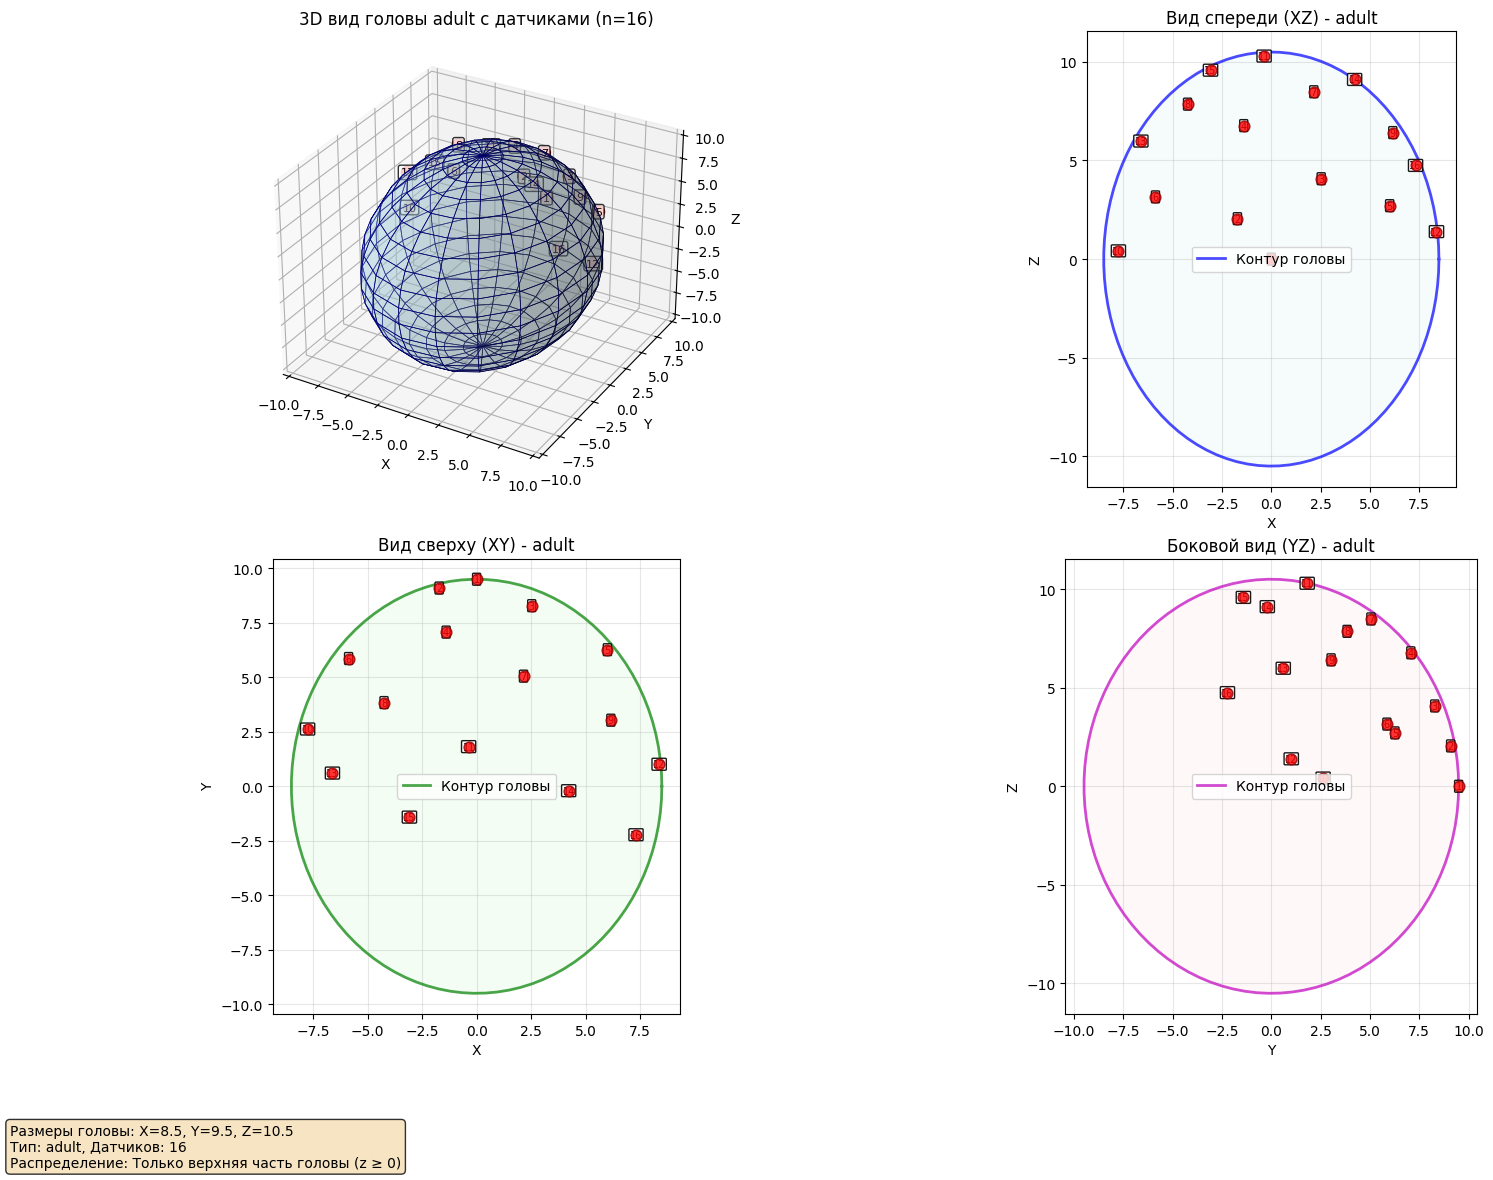
\includegraphics[width=0.6\textwidth]{../../figures/synthetic_head_views.png}
\caption{Визуализация синтетической модели головы с расположением датчиков и источников.}
\label{fig:synthetic_head_views}
\end{figure}

Синтетические данные позволяют оценить точность восстановления как на поверхности (Sensor MSE), так и во внутренней области (Deep MSE). Результаты эксперимента представлены в таблице \ref{tab:synthetic_results}.

\begin{table}[h]
\centering
\begin{tabular}{lccr}
\hline
Метод & Sensor MSE & Deep MSE & Примечания \\
\hline
Предложенный метод & --- & --- & Включает энергетическую и TV-регуляризацию \\
LORETA & --- & --- & Стандартная реализация \\
\hline
\end{tabular}
\caption{Сравнение методов по синтетическим данным.}
\label{tab:synthetic_results}
\end{table}

Результаты синтетического эксперимента подтверждают, что предложенный метод обеспечивает более точное восстановление полей и источников во внутренней области $\Omega$ (Deep MSE) по сравнению с LORETA, сохраняя при этом сопоставимую точность на датчиках. Это объясняется использованием энергетической регуляризации $\mathcal{R}_E(s)$, которая учитывает физические принципы взаимодействия поля с источниками, и TV-регуляризации $\mathcal{R}_{TV}(s)$, способствующей локализации источников.

\section{Результаты}
\label{subsec:discussion}
Энергетическая регуляризация $\mathcal{R}_E(s) = \langle Ts, s \rangle_{\mathcal{S}}$ обеспечивает устойчивость решения обратной задачи даже при вырожденном операторе наблюдения $K$. Это подтверждается сопоставимыми значениями Sensor MSE для предложенного метода и LORETA на реальных данных.
TV-регуляризация $\mathcal{R}_{TV}(s)$ способствует локализации источников и подавлению нефизичных осцилляций, что приводит к улучшению точности восстановления во внутренней области $\Omega$ на синтетических данных.
Адаптивная настройка параметра $\lambda_{\mathrm{data}}$ позволяет балансировать между точностью аппроксимации данных и устойчивостью решения, что особенно важно для реальных данных с высоким уровнем шума.
Таким образом, предложенный метод демонстрирует высокую эффективность в решении обратной задачи ЭЭГ, обеспечивая устойчивое и физически обоснованное восстановление распределения источников сигнала.
 Сочетание энергетической и TV-регуляризации позволяет преодолеть ограничения существующих подходов, таких как LORETA, и получить более точные результаты в условиях ограниченного 
 числа датчиков и высокого уровня шума.

Недостатки предложенного метода включают повышенную вычислительную сложность по сравнению с LORETA, что связано с необходимостью решения более сложной оптимизационной задачи. 
Кроме того, выбор параметров регуляризации $\alpha$ и $\beta$ может требовать дополнительной настройки для достижения оптимальных результатов на различных наборах данных. Наличие регуляризатора 
$\mathcal{R}_E(s)$ может ограничивать применимость метода к задачам, где оператор $T$ не соответствует физическим принципам взаимодействия поля с источниками. Таже регулризатор смещает решение 
в сторону источников с меньшей энергией, что может не всегда соответствовать реальной физиологии мозга.

\bibliography{npde-bibliography}

\end{document}
